\Section{Быстрое преобразование Фурье}{4 декабря 2017}{Сергей Копелиович}

\down
Перед тем, как начать говорить ``Фурье'' то, ``Фурье'' сё, нужно сразу заметить:

Есть \href{https://ru.wikipedia.org/wiki/%D0%9F%D1%80%D0%B5%D0%BE%D0%B1%D1%80%D0%B0%D0%B7%D0%BE%D0%B2%D0%B0%D0%BD%D0%B8%D0%B5_%D0%A4%D1%83%D1%80%D1%8C%D0%B5}{непрерывное преобразование Фурье}. С ним вы должны столкнуться на теорвере.

Есть \href{https://ru.wikipedia.org/wiki/%D0%A0%D1%8F%D0%B4_%D0%A4%D1%83%D1%80%D1%8C%D0%B5}{тригонометрический ряд Фурье}.
И есть общий ряд Фурье в гильбертовом пространстве, который появляется в начале курса функционального анализа.

Мы же с вами будем заниматься исключительно \href{https://ru.wikipedia.org/wiki/%D0%94%D0%B8%D1%81%D0%BA%D1%80%D0%B5%D1%82%D0%BD%D0%BE%D0%B5_%D0%BF%D1%80%D0%B5%D0%BE%D0%B1%D1%80%D0%B0%D0%B7%D0%BE%D0%B2%D0%B0%D0%BD%D0%B8%D0%B5_%D0%A4%D1%83%D1%80%D1%8C%D0%B5}{дискретным преобразованием Фурье}. \\
Коротко DFT (Discrete Fourier transform). FFT -- по сути то же, первая буква означает ``fast''.

\down
{\bf Задача:} даны два многочлена $A$, $B$ суммарной длины $\le n$, переменожить их за $\O(n \log n)$.

\down
Длина многочлена -- $\gamma(A) = (\deg A) + 1$. Вводим её, чтобы везде не писать ``${-}1$''.

Если даны $n$ точек $(x_i, y_i)$, все $x_i$ различны, $\exists !$
интерполяционный многочлен длины $n$, построенный по этим точкам (из алгебры).
Ещё заметим: $\gamma(AB) = \gamma(A) + \gamma(B) - 1$. Наш план: 

\up
\hspace*{-0.5em}\begin{tabular}{ll}
\parbox{15cm}{
	\begin{MyList}[0pt]
	\item Подобрать удачные $k$ и точки $w_0, w_1, \dots, w_{k-1} \colon k \ge \gamma(A) + \gamma(B) - 1 = n$.
	\item Посчитать значения $A$ и $B$ в $w_i$.
	\item $AB(x_i) = A(x_i)B(x_i)$. Эта часть самая простая, работает за $\O(n)$.
	\item Интерполировать $AB$ длины $k$ по полученным парам $\q{w_i, AB(w_i)}$.
	\end{MyList}

	\up
	{\bf Вспомним комплексные числа: }

	\down
	$e^{2\pi i \alpha}e^{2\pi i \beta} = e^{2\pi i(\alpha{+}\beta)}$
	$e^{2\pi i \PHI} = (\cos \PHI, \sin \PHI)$, $\overline{(a, b)} = (a, -b)$
	$\SO \overline{e^{2\pi i \PHI}} = e^{2\pi i(-\PHI)}$

	Извлечение корня $k$-й степени: $\sqrt[k]{z} = \sqrt[k]{e^{2\pi i \PHI}} = e^{2\pi i \PHI / k}$

	Если взять все корни из $1$ степени $2^t$, возвести в квадрат, \\
	получатся ровно все корни степени $2^{t-1}$. Корни из $1$ степени $k$: $e^{2\pi i j / k}$.
}
&
\parbox{10cm}{
	\vspace*{1.5em}
	\hspace*{-2.5em}
	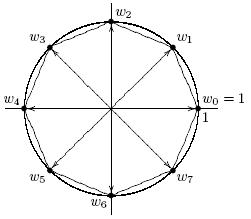
\includegraphics[width=120pt]{pics/fft_roots.jpg}
} \\
\end{tabular}

\Subsection{Прелюдия к FFT}

Возьмём $\min N = 2^t \ge n$ и $w_j = e^{2\pi i j / N}$. 
Тут мы предполагаем, что $A, B \in \mathbb{C}[x]$ или $A, B \in \R[x]$.

Пусть есть многочлены $A(x) = \sum a_i x^i$ и $B(x) = \sum b_i x^i$. Ищем $C(x) = A(x)B(x)$.

Обозначим их значения в точках $w_0, w_1, \dots, w_{k-1} \colon A(w_i) = fa_i, B(w_i) = fb_i, C(w_i) = fc_i$.

% Значения $C(x) = A(x)B(x)$ в точках $x_i$ можно получить за линейное время: 

% \begin{smallformula}
% $$fc_i = C(x_i) = A(x_i)B(x_i) = fa_ifb_i$$
% \end{smallformula}

Схема быстрого умножения многочленов: 

\begin{smallformula}
$$a_i, b_i \overset{\O(n \log n)}{\longrightarrow} fa_i, fb_i \overset{\O(n)}{\longrightarrow} fc_i = fa_ifb_i \overset{\O(n \log n)}{\longrightarrow} c_i$$
\end{smallformula}

% Осталось подобрать правильные точки $x_i$.

% \down
% FFT расшифровывается Fast Fourier Transform и за $\O(n \log n)$ вычисляет значения многочлена в точках $w_j = e^{\mfrac{2\pi i j}{n}}$ для
% $n = 2^k$ (то есть, только для степеней двойки).

\up
\Subsection{Собственно идея FFT}

$A(x) = \sum a_i x^i = (a_0 + x^2a_2 + x^4a_4 + \dots) + x(a_1x + a_3x^3 + a_5x^5 + \dots) = P(x^2) + xQ(x^2)$\\
Т.е. обозначили все чётные коэффициенты $A$ многочленом $P$, а нечётные соответственно $Q$.

\down
$\gamma(A) = n$, все $w_j^2 = w_{n/2+j}^2 \SO$ многочлены $P$ и $Q$ нужно считать не в $n$, а в $\mfrac{n}{2}$ точках.

\down
\begin{codep}
def FFT(a): 
  n = len(a)
  if n == 1: return a[0] # `посчитать значение A(x) = a[0] в точке 1`
  a ---> p, q # `разбили коэффициенты на чётные и нечётные`
  p, q = FFT(p), FFT(q) 
  w = exp(2pi*i/n) # `корень из единицы $n$-й степени`
  for i=0..n-1: a[i] = p[i%(n/2)] + w`$\black{^\t{i}}$`*q[i%(n/2)]
  return a
\end{codep}

Время работы $T(n) = 2T(n/2) + \O(n) = \O(n \log n)$.

\Subsection{Крутая реализация FFT}

Чтобы преобразование работало быстро, нужно заранее предподсчитать все $w_j = e^{2\pi i j / N}$.

Заметим, что $p$ и $q$ можно хранить прямо в массиве $a$.\\
Тогда получается, что на прямом ходу рекурсии мы просто переставляем местами элементы $a$, и только на обратном делаем какие-то полезные действия.\\
Число $a_i$ перейдёт на позицию $a_{rev(i)}$, где $rev(i)$ -- перевёрнутая битовая запись~$i$. \\
Кстати, $rev(i)$ мы уже умеем считать динамикой для всех~$i$.

При реализации на \t{C++} можно использовать комплексные числа из STL: \t{complex<double>}.

\begin{code}
const int K = 20, N = 1 << K;
complex<double> root[N];
int rev[N];
void init() {
	for (int j = 0; j < N; j++) {
		root[j] = exp(2`$\color{black}{\pi}$`*i*j/N); // `$\cos(2\pi j/N), \sin(2\pi j/N)$`
		rev[j] = (rev[j >> 1] >> 1) + ((j & 1) << (K - 1));
	}
}
\end{code}

Теперь, корни из единицы степени $k$ хранятся в \t{root[j*N/k]}, $j \in [0,k)$. Две проблемы: \\
1. Доступ к памяти при этом не последовательный, проблемы с кешом.\\
2. Мы $2N$ раз вычисляли тригонометрические функции.\\
$\SO$ можно лучше, вычисления корней \NO{2}:

\begin{code}
for (int k = 1; k < N; k *= 2) {
	num tmp = exp(`\color{black}{$\pi$}`/k);
	root[k] = {1, 0}; // `в root[k..2k) хранятся первые k корней степени 2k`
	for (int i = 1; i < k; i++)
		root[k + i] = (i & 1) ? root[(k + i) >> 1] * tmp : root[(k + i) >> 1];
}
\end{code}

Теперь код собственно преобразования Фурье может выглядеть так:

\begin{code}
void FFT(a, fa) { // a --> fa
  for (int i = 0; i < N; i++)
    fa[rev[i]] = a[i]; // `можно иначе, но давайте считать массив <<\t{a}>> readonly`
  for (int k = 1; k < N; k *= 2) // `уже посчитаны FFT от кусков длины k, база: k=1`
    for (int i = 0; i < N; i += 2 * k) // `[i..i+k) [i+k..i+2k) ---> [i..i+2k)`
      for (int j = 0; j < k; j++) { // `оптимально написанный стандартный цикл FFT`
        num tmp = root[k + j] * fa[i + j + k]; // `вторая версия root[]`
        fa[i + j + k] = fa[i + j] - tmp; // `exp(${2\pi i(j{+}n/2)/n}$) = {-}exp(${2\pi i j / n}$)`
        fa[i + j] = fa[i + j] + tmp;
      }
}
\end{code}

\pagebreak
\vspace*{-1.5em}
\Subsection{Обратное преобразование}

Теперь имея при $w = e^{2 \pi i / n}$:

$fa_0 = a_0 + a_1 + a_2 + a_3 + \dots$

$fa_1 = a_0 + a_1w + a_2w^2 + a_3w^3 + \dots$

$fa_2 = a_0 + a_1w^2 + a_2w^4 + a_3w^3 + \dots$

$\dots$

Нам нужно научиться восстанавливать коэффициенты $a_0, a_1, a_2, \dots$, имея только $fa_i$.

Заметим, что $\forall j \not= 0 \ \sum\limits_{k=0}^{n-1} w^{jk} = 0$ (геометрическая прогрессия). А при $j = 0$ получаем $\sum\limits_{k=0}^{n-1} w^{jk} = n$.

\down
Поэтому $fa_0 + fa_1 + fa_2 + \dots = a_0n + a_1\sum_k w^k + a_2 \sum_k w^{2k} + \dots = a_0n$

Аналогично $fa_0 + fa_1w^{-1} + fa_2w^{-2} + \dots = \sum_k a_0 w^{-k} + a_1n + a_2 \sum_k w^{k} + \dots = a_1n$

И в общем случае $\sum_k fa_kw^{-jk} = a_jn$. 

Заметим, что это ровно значение многочлена с коэффициентами $fa_k$ в точке $w^{-j}$.

Осталось заметить, что множества чисел $\{w_j\,|\,j=0..n{-}1\}$ и $\{w_{-j}\,|\,j=0..n{-}1\}$ совпадают $\SO$

\down
\begin{code}
void FFT_inverse(fa, a) { // fa --> a
  FFT(fa, a)
  reverse(a + 1, a + N) // w^j <--> w^{-j}
  for (int i = 0; i < N; i++) a[i] /= N;
}
\end{code}

%\pagebreak
%\vspace*{-1.5em}
\Subsection{Два в одном}

Часто коэффициенты многочленов -- вещественные числа. \\
Если у нас есть многочлены $A(x), B(x) \in \mathbb{R}[x]$,
возьмём числа $c_j = a_j + ib_j$ и \\ 
посчитаем $fc = FFT(c)$.
Тогда по $fc$ за $\O(n)$ можно легко восстановить $fa$ и $fb$.

\down
Для этого вспомним про сопряжения комплексных чисел: \\
$\overline{x + iy} = x - iy, \overline{a \cdot b} = \overline{a} \cdot \overline{b}, w^{n-j} = w^{-j} = \overline{w^j} \SO
\overline{fc_{n-j}} = \overline{C(w^{n-j})} = \overline{C}(w^j) \SO$\\
$fc_j + \overline{fc_{n-j}} = 2 \cdot A(w^j) = 2 \cdot fa_j$. Аналогично $fc_j - \overline{fc_{n-j}} = 2i \cdot B(w^j) = 2i \cdot fb_j$.

\down
Теперь, например, для умножения двух $\R[x]$ можно использовать не $3$ вызова FFT, а $2$.

\Subsection{Умножение чисел, оценка погрешности}

Общая схема умножения чисел: \\
цифра -- коэффициент многочлена ($x = 10$); умножим многочлены; сделаем переносы.

\down
Число длины $n$ в системе счисления $10$ можно за $\O(n)$ перевести в систему счисления $10^k$.
Тогда многочлены будут длины $n/k$, умножение многочленов работать за $\mfrac{n}{k}\log\mfrac{n}{k}$ (убывает от $k$).\\
Возникает вопрос, какое максимальное $k$ можно использовать?\\
Коэффициенты многочлена-произведения будут целыми числами до $(10^k)^2 \mfrac{n}{k}$.\\ 
Чтобы в типе \t{double} целое число хранилось с погрешностью меньше $0.5$ (тогда его можно правильно округлить к целому),
оно должно быть не более $10^{15}$. \\
Получаем при $n \le 10^6$, что $(10^k)^2 10^6 / k \le 10^{15} \SO k \le 4$.\\
Аналогично для типа \t{long double} имеем $(10^k)^2 10^6 / k \le 10^{18} \SO k \le 6$.\\
Это оценка сверху, предполагающая, что само FFT погрешность не накапливает... на самом деле эта оценка очень близка к точной.
